\chapter{Methods}
%\addcontentsline{toc}{chapter}{2. Methods}
This experiment was granted ethics approval from the Western University Non-Medical Research Ethics Board. 
The approval form can be found in Appendix \ref{appendix:ethics}.
\section{Participants}
Fourteen participants (3 male), aged 19-36, with normal hearing and no history of brain injury took part in this study. Eight participants had formal musical training (1- 26 years), and four of the participants played instruments regularly at the time of data collection.
\section{Stimuli}
Stimuli were fragments of familiar musical pieces and were selected based on key signature (3/4 or 4/4 time) and the presence and absence of lyrics. The stimuli were kept as similar in length as possible with care taken to ensure that they all contained complete musical phrases. Stimulus details can be found in \autoref{tab:stimuli_information}.
Each musical fragment was preceded by approximately two seconds of clicks as a cue to the tempo and onset of the music. The beats began to fade out at the one second mark and stopped at the onset of the music. 

\section{Equipment and Procedure}
\subsection{Behavioural Testing}
We collected information about the participants' previous music experience, their ability to imagine sounds, and information about musical sophistication using an adapted version of the widely used Goldsmith's Musical Sophistication Index (G-MSI) \cite{mullensiefen_musicality_2014} combined with an adapted clarity of auditory imagination scale \cite{willander_imagery_scale_2010}. 
The questionnaire can be found in Appendix \ref{appendix:questionnaire}.
Participants also completed a beat tapping and a stimuli familiarity task. 
Participants listened to each stimulus and tapped along with the music on the table top. 
Participants'  tapping abilities were rated on a scale from 1 (difficult to assess) to 3 (tapping done properly). 
After listening to each stimulus participants rated their familiarity with the stimuli on a scale from 1 (unfamiliar) to 3 (very familiar).
To participate in the \ac{EEG} portion of the study, the participants had to receive a score of at least 90\% on the beat tapping task to ensure that they could adequately maintain a steady beat.
Participants received scores from 75\%--100\% with an average score of 96\%.
Furthermore, they needed to receive a score of at least 80\% on our stimuli familiarity task. 
This measure ensured that participants were familiar with the stimuli and imagination was as easy as possible. 
Participants received scores from 71\%--100\% with an average score of 87\%.
These requirements resulted in rejecting 4 participants.
This left 10 participants (3 male), aged 19--36, with normal hearing and no history of brain injury. 
These 10 participants had an average tapping score of 98\% and an average familiarity score of 92\%.
Eight participants had formal musical training (1--10 years), and four of those participants played instruments regularly at the time of data collection.

\begin{table}[t]
\small
%\setlength{\tabcolsep}{2.5pt}  % use to control space between columns
%\renewcommand{\arraystretch}{1}
\centering
\caption{Tempo, meter and length of the stimuli used in the beat-tapping and stimuli-familiarity experiment.}
%Mean and standard deviation over individual subjects.}
\label{tab:stimuli_information}
%{\footnotesize % \sffamily \fontfamily{anttlc}\selectfont
%{\small % \sffamily \fontfamily{anttlc}\selectfont
\begin{tabularx}{\columnwidth}{r l c c  c c c }
\toprule
ID		& Name							&Meter 	& Length	& Tempo 		&\#Bars	& Bar Length\\
\midrule
1		& Chim Chim Cheree (lyrics)			& 3/4		& 13.3s 			& 212 BPM 	& 16				& 0.85s	\\ 
2		& Take Me Out to the Ballgame (lyrics)	& 3/4		& 7.7s 			& 189 BPM 	& 8				& 0.95s	\\ 
3		& Jingle Bells (lyrics)					& 4/4		& 9.7s 			& 200 BPM 	& 8				& 1.20s	\\ 
4		& Mary Had a Little Lamb (lyrics)		& 4/4		& 11.6s			& 160 BPM 	& 8				& 1.50s	\\ 
11		& Chim Chim Cheree 				& 3/4		& 13.5s	 		& 212 BPM 	& 16				& 0.85s	\\ 
12		& Take Me Out to the Ballgame			& 3/4		& 7.7s 			& 189 BPM 	& 8				& 0.95s	\\ 
13		& Jingle Bells 						& 4/4		& 9.0s 			& 200 BPM 	& 8				& 1.20s	\\ 
14		& Mary Had a Little Lamb				& 4/4		& 12.2s			& 160 BPM 	& 8				& 1.50s	\\ 
21		& Emperor Waltz					& 3/4		& 8.3s 			& 178 BPM 	& 8				& 1.01s	\\ 
22		& Hedwig's Theme (Harry Potter)		& 3/4		& 16.0s	 		& 166 BPM 	& 15				& 1.08s	\\
23		& Imperial March (Star Wars Theme)		& 4/4		& 9.2s 			& 104 BPM 	& 4				& 2.30s	\\ 
24		& Eine Kleine Nachtmusik				& 4/4		& 6.9s			& 140 BPM 	& 4				& 1.71s	\\
\bottomrule
\end{tabularx}
%}
\end{table}


\subsection{EEG recording}
For the EEG portion of the study, the 10 participants sat in an audiometric room (Eckel model CL-13) and connected to a BioSemi Active-Two system recording 64+2 EEG channels at 512 Hz as shown in \autoref{fig:eegsetup}.
\begin{figure}[htb]
  \begin{center}
    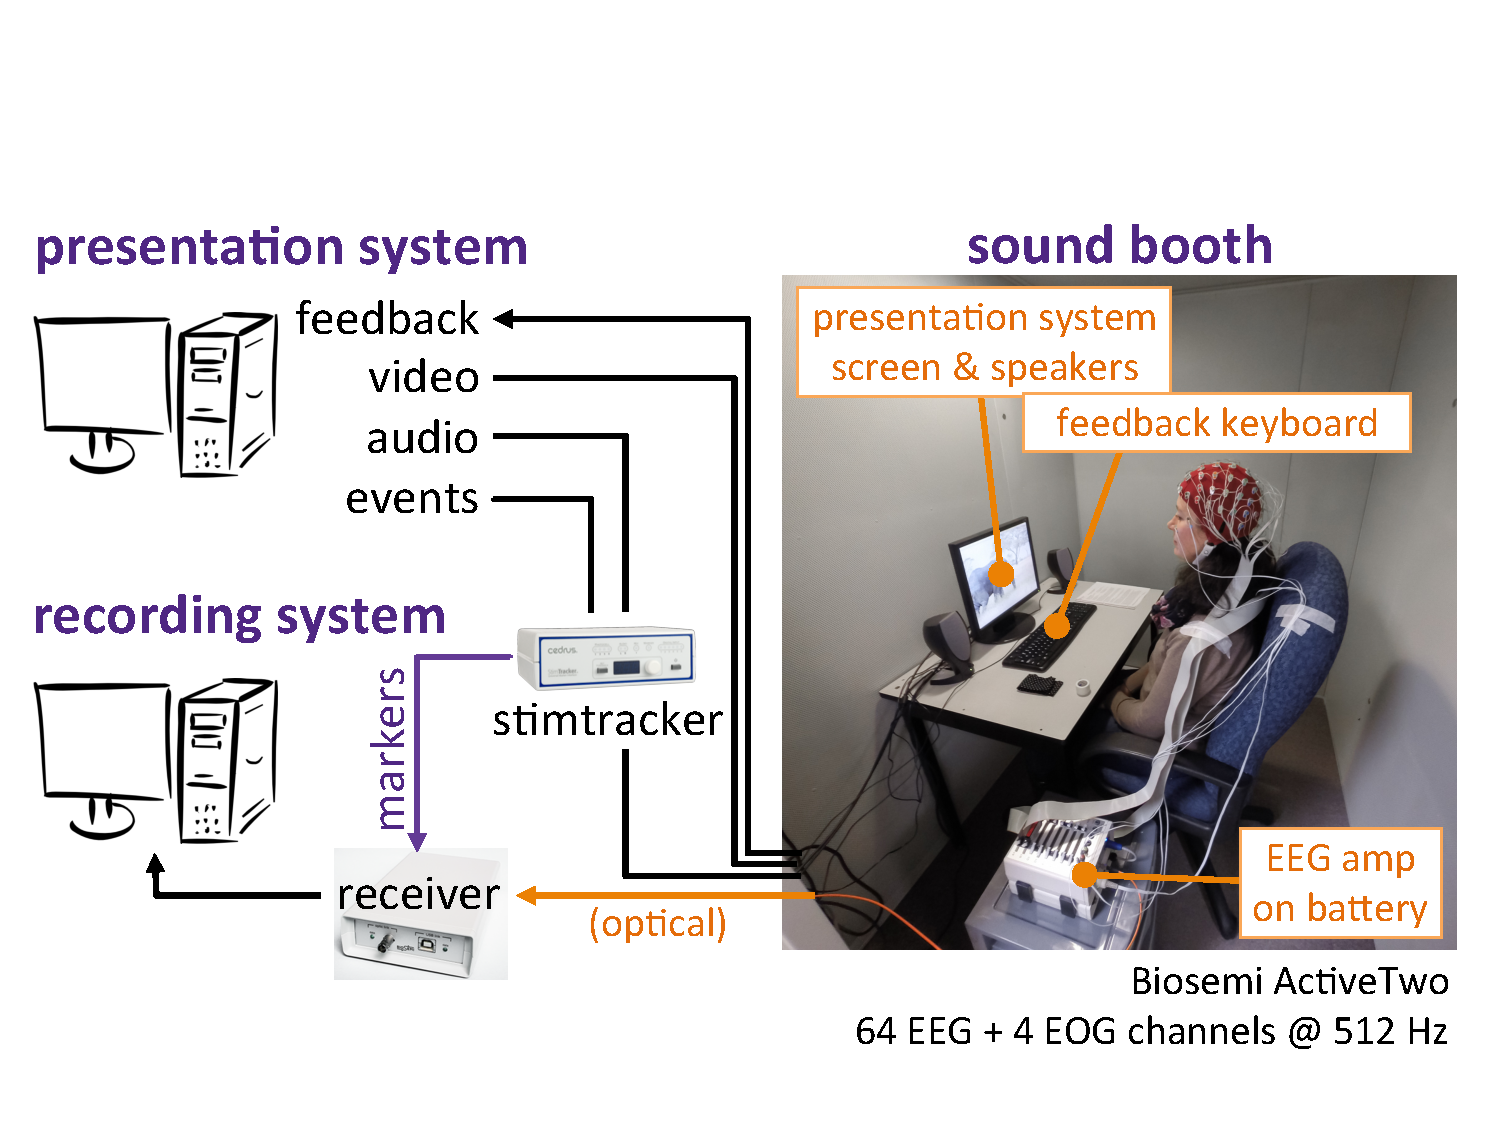
\includegraphics[scale=0.48]{Figures/EEG-setup.pdf}
%   \\\vspace{-0.8em}
    \caption{%
Setup for the EEG experiment.
The presentation and recording systems were placed outside to reduce the impact of electrical line noise that could be picked up by the EEG amplifier.
}
    \label{fig:eegsetup}
  \end{center}
% \vspace{-2em}
\end{figure}
Horizontal and vertical EOG channels recorded eye movements. 
We also recorded the left and right mastoid channel as EEG reference signals. 
Due to an oversight, the mastoid data were not collected for the first five subjects.
In these subjects data was 
The presented audio %and the recorded EEG were 
was routed through a Cedrus StimTracker connected to the EEG receiver, which allowed a high-precision synchronization ($<$0.05 ms) of the stimulus onsets with the \ac{EEG} data.
The experiment was programmed and presented using PsychToolbox run in Matlab 2014a. 
A computer monitor displayed the instructions and fixation cross for the participants to focus on during the trials to reduce eye movements.
The stimuli and cue clicks were played through speakers at a comfortable volume that was kept constant across participants. Headphones were not used because pilot participants reported headphones caused them to hear their heartbeat which interfered with the imagination portion of the experiment. 
After the experiment, we asked participants the method they used to imagine music. 
The participants were split evenly between imagining themselves producing the music (singing or humming) and simply ``hearing the music in [their] head.'' 

The EEG experiment was divided into 2 parts with 5 blocks each as illustrated in \autoref{fig:experiment_outline}.
\begin{figure}[htbp]
  \begin{center}
    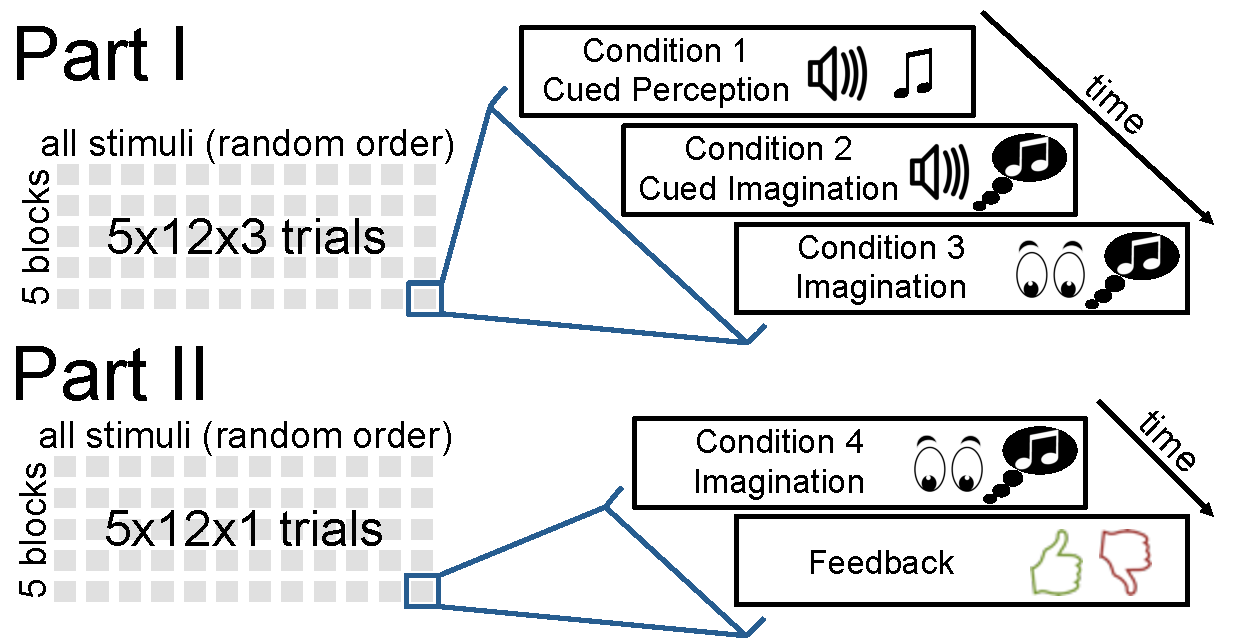
\includegraphics[scale=0.6]{Figures/study_design_small.pdf}
    \caption{%
Illustration of the design for the EEG portion of the study.
}
    \label{fig:experiment_outline}
  \end{center}
\end{figure}
A single block comprised all 12 stimuli in randomized order.
Between blocks, participants could take breaks at their own pace.
We recorded EEG in 4 conditions:
\begin{enumerate}
\item
Stimulus perception preceded by cue clicks
\item
Stimulus imagination preceded by cue clicks
\item
Stimulus imagination without cue clicks
\item
Stimulus imagination without cue clicks, with feedback
\end{enumerate}

The goal was to use the cue to align trials of the same stimulus collected under conditions 1 and 2. Lining up the trials allows us to directly compare the perception and imagination of music and to identify overlapping features in the data. 
Conditions 3 and 4 simulate a more realistic query scenario during which the system does not have prior information about the tempo and meter of the imagined stimulus.
Conditions 3 and 4 were identical except for the trial context.
While the condition 1--3 trials were recorded directly back-to-back within the first part of the experiment, 
all condition 4 trials were recorded separately in the second part without any cue clicks or tempo priming by prior presentation of the stimulus.
After each condition 4 trial, participants provided feedback by pressing one of two buttons indicating whether or not they felt they had imagined the stimulus correctly.
In total, 240 trials (12 stimuli x 4 conditions x 5 blocks) were recorded per subject.

\section{Preprocessing}
The raw EEG and EOG data were processed using the MNE-Python toolbox. 
For recordings with additional mastoid channels, the EEG data was re-referenced by subtracting the mean mastoid signal \cite{teplan_fundamentals_2002}.
We then removed and interpolated bad EEG channels identified by manual visual inspection. 
Channels containing noise that could not be removed using simple filtering techniques were labeled as bad. 
For interpolation, the spherical splines method described in \cite{perrin_spherical_1989} was applied.
The data were then filtered with an fft-bandpass, keeping a frequency range between 0.5 and 30 Hz.
This removed unwanted high frequency information and any slow signal drift in the EEG.
Removing unwanted noise removes signals originating from external sources, and allows analyses to be done on data within the frequency range of signals produced by the brain. 
%Afterwards, we down-sampled to a sampling rate of 64 Hz.
To remove artifacts caused by eye blinks, we computed independent components using extended Infomax \ac{ICA} \cite{lee_independent_1999} and semi-automatically removed components that had a high correlation with the EOG channels.
Finally, the 64 EEG channels were reconstructed from the remaining independent components.